% This is "sig-alternate.tex" V2.1 April 2013
% This file should be compiled with V2.5 of "sig-alternate.cls" May 2012
%
% This example file demonstrates the use of the 'sig-alternate.cls'
% V2.5 LaTeX2e document class file. It is for those submitting
% articles to ACM Conference Proceedings WHO DO NOT WISH TO
% STRICTLY ADHERE TO THE SIGS (PUBS-BOARD-ENDORSED) STYLE.
% The 'sig-alternate.cls' file will produce a similar-looking,
% albeit, 'tighter' paper resulting in, invariably, fewer pages.
%
% ----------------------------------------------------------------------------------------------------------------
% This .tex file (and associated .cls V2.5) produces:
%       1) The Permission Statement
%       2) The Conference (location) Info information
%       3) The Copyright Line with ACM data
%       4) NO page numbers
%
% as against the acm_proc_article-sp.cls file which
% DOES NOT produce 1) thru' 3) above.
%
% Using 'sig-alternate.cls' you have control, however, from within
% the source .tex file, over both the CopyrightYear
% (defaulted to 200X) and the ACM Copyright Data
% (defaulted to X-XXXXX-XX-X/XX/XX).
% e.g.
% \CopyrightYear{2007} will cause 2007 to appear in the copyright line.
% \crdata{0-12345-67-8/90/12} will cause 0-12345-67-8/90/12 to appear in the copyright line.
%
% ---------------------------------------------------------------------------------------------------------------
% This .tex source is an example which *does* use
% the .bib file (from which the .bbl file % is produced).
% REMEMBER HOWEVER: After having produced the .bbl file,
% and prior to final submission, you *NEED* to 'insert'
% your .bbl file into your source .tex file so as to provide
% ONE 'self-contained' source file.
%
% ================= IF YOU HAVE QUESTIONS =======================
% Questions regarding the SIGS styles, SIGS policies and
% procedures, Conferences etc. should be sent to
% Adrienne Griscti (griscti@acm.org)
%
% Technical questions _only_ to
% Gerald Murray (murray@hq.acm.org)
% ===============================================================
%
% For tracking purposes - this is V2.0 - May 2012

\documentclass{sig-alternate-05-2015}
\usepackage{graphicx}
\usepackage{underscore}


\begin{document}

% Copyright

%\setcopyright{acmlicensed}
%\setcopyright{rightsretained}
%\setcopyright{usgov}
%\setcopyright{usgovmixed}
%\setcopyright{cagov}
%\setcopyright{cagovmixed}




%Conference

%
% --- Author Metadata here ---
%\CopyrightYear{2007} % Allows default copyright year (20XX) to be over-ridden - IF NEED BE.
%\crdata{0-12345-67-8/90/01}  % Allows default copyright data (0-89791-88-6/97/05) to be over-ridden - IF NEED BE.
% --- End of Author Metadata ---

\title{Evaluation of Indexing Techniques for Geo-spatial Data}
\subtitle{[CSE591: Advances in Databases]}
%
% You need the command \numberofauthors to handle the 'placement
% and alignment' of the authors beneath the title.
%
% For aesthetic reasons, we recommend 'three authors at a time'
% i.e. three 'name/affiliation blocks' be placed beneath the title.
%
% NOTE: You are NOT restricted in how many 'rows' of
% "name/affiliations" may appear. We just ask that you restrict
% the number of 'columns' to three.
%
% Because of the available 'opening page real-estate'
% we ask you to refrain from putting more than six authors
% (two rows with three columns) beneath the article title.
% More than six makes the first-page appear very cluttered indeed.
%
% Use the \alignauthor commands to handle the names
% and affiliations for an 'aesthetic maximum' of six authors.
% Add names, affiliations, addresses for
% the seventh etc. author(s) as the argument for the
% \additionalauthors command.
% These 'additional authors' will be output/set for you
% without further effort on your part as the last section in
% the body of your article BEFORE References or any Appendices.

\numberofauthors{3} %  in this sample file, there are a *total*
% of EIGHT authors. SIX appear on the 'first-page' (for formatting
% reasons) and the remaining two appear in the \additionalauthors section.
%
\author{
% You can go ahead and credit any number of authors here,
% e.g. one 'row of three' or two rows (consisting of one row of three
% and a second row of one, two or three).
%
% The command \alignauthor (no curly braces needed) should
% precede each author name, affiliation/snail-mail address and
% e-mail address. Additionally, tag each line of
% affiliation/address with \affaddr, and tag the
% e-mail address with \email.
%
% 1st. author
\alignauthor
Karthik Ramesh\\
       \affaddr{CIDSE ASU}\\
       \email{kramesh3@asu.edu}
% 2nd. author
\alignauthor
Sidharth Ramesh\\
       \affaddr{CIDSE ASU}\\
       \email{sramesh8@asu.edu}
% 3rd. author
\alignauthor Vignesh Natarajan\\
       \affaddr{CIDSE ASU}\\
       \email{vignesh.natarajan@asu.edu}
}
% There's nothing stopping you putting the seventh, eighth, etc.
% author on the opening page (as the 'third row') but we ask,
% for aesthetic reasons that you place these 'additional authors'
% in the \additional authors block, viz.
%\date{30 July 1999}
% Just remember to make sure that the TOTAL number of authors
% is the number that will appear on the first page PLUS the
% number that will appear in the \additionalauthors section.

\maketitle
\begin{abstract}
Spatial indices play a vital role in spatial query processing. The performance of spatial queries such as kNN, spatial joins, range query, containment query etc. depends much on the type of spatial index that is used on the data. In this paper we provide a comparative study of different indexing techniques that are applied to spatial data. We compare the performance of four indexing techniques, namely GiST(Generalized Search Tree), B-Tree, k-d tree and Quadtree. Specifically, we apply different indexing techniques on a data set consisting of point data type and do a comparative study on the performance of these indices for different query types. The study will provide the reader an opportunity to select the most suitable index based on the query types that are frequent in their application.
\end{abstract}


%
% The code below should be generated by the tool at
% http://dl.acm.org/ccs.cfm
% Please copy and paste the code instead of the example below. 
%

%
% End generated code
%

%
%  Use this command to print the description
%

% We no longer use \terms command
%\terms{Theory}


\section{Introduction}
With an explosion in the amount of data generation from a multitude of originating points like mobile, GPS, and budding areas like the Internet of Things, it becomes imperative to understand how databases have evolved around these advancements. One of the primary metrics used to evaluate the efficiency of a database is speed. Particularly, the problem of optimizing the speed at which records can be located or retrieved, is one of enormous interest. The database component that deals with this aspect is the database index.\\

In this project we propose to evaluate different techniques used to build this particular component of a database. Database indexing techniques have been studied extensively and several classifications of the prominent types of database indexing techniques have been proposed in the past. With the amount of geospatial data available, it is of interest to study different techniques to index the same. In this project, we take one such taxonomy of geospatial data indexing and study how methods in each indexing category work differently on a database when indexing spatial data. For this purpose, we expect to choose a representative indexing method under each category of the taxonomy, a sample dataset(s), and document the results of some of the standard spatial queries from those specified by the Open Geospatial Consortium Standard \cite{ogc}. Some examples of which are \cite{wiki:spatial}:
\begin{itemize}
\item \textbf{Spatial Measurements}: Computing length, polygon area, the distance between geometries etc.
\item \textbf{Spatial Functions}: Modify existing features to create new ones, for example by providing a buffer around them, intersecting features etc.
\item \textbf{Spatial Predicates}: Allow true/false queries about spatial relationships between geometries.
\item \textbf{Geometry Constructors}: Creates new geometries, usually by specifying vertices which define the shape.
\item \textbf{Observer Functions}: Queries which return specific information about the feature such as location of the center of a circle.
\end{itemize}

The idea is to evaluate the performance of the multiple indexing methods that perform spatial data processing. Various data structures are used for indexing methods in several relational databases. For instance, B$^{-}$ - Tree on Microsoft SQL Server, R-Tree in PostgreSQL/MySQL, Quad-Tree in Oracle Spatial database, and R$^{*}$-Tree in SQLite.\\

We present the results comparing the indexing methods on a geolocation dataset such as the one available in \cite{sarwat:data}. The goal of this experiment is to understand which indexing method performs best on the aforementioned types of spatial queries given a data set and a relational database. We can surmise that different index types are suited for different types of spatial queries and we hope to present analyses which would benefit readers to select index type based on the type of queries which they believe would be most used in their application. The dataset we propose to use is PostgreSQL. The choice of the database is because of its ability to provide all the indexing methods we plan to evaluate.\\

The motivation behind this evaluation experiment is the growing interest in leveraging geospatial data processing, and interest in huge data sets of popular location based products like Uber and FourSquare. Efficient indexing is of interest for these applications as faster look up would mean the apps can scale much better and existing RDBMS can be leveraged to perform the necessary spatial computations. \\

\section{Literature Review}

\subsection{Spatial Data and the need for indexing}
Spatial data is the kind of data that has to do with spatial co-ordinates -- meaning they exist in space. The most common types of queries that need to be answered when it comes to dealing with this type of data fall into two types - intersection, and containment. For instance, if you have the spatial description of a state, questions like whether or not a particular city (given its spatial description) lies within the state can be answered. This is a containment query. Similarly, given the spatial description of two states, intersection queries can help answering whether or not the states share common borders. 

An extensive description (and one of the earliest definitions) of spatial data, the challenges in representing spatial data, and the types of spatial data systems was presented by \cite{guting1994introduction}. The paper states that there are two things that primarily require representation when dealing with spatial data:
\begin{itemize}
\item \textit{Objects in Space:} Entities that have their own geometric description -- points, lines.
\item \textit{Space itself:} A representation of the collection as a whole. 
\end{itemize}

Querying when dealing with spatial data is essentially connecting the operations of spatial algebra (including relations) to traditional database queries. Among these operations on spatial data, \textit{spatial relationships} are the most important operations, and those are the ones that need mapping to query operations possible using traditional databases. Operations such as nearest neighbors, all objects within a window etc., fall under this category of spatial relationships. Several classes of such relationships have been identified in available literature \cite{pullar1988toward}, \cite{egenhofer1989formal}, \cite{worboys1992generic}:

\begin{itemize}
\item \textbf{\textit{Topological Relationships:}} Relationships such as whether co-ordinates (or co-ordinate sets) are adjacent and disjoint, are invariant under topological transformations like translation or scaling.
\item \textbf{\textit{Direction Relationships:}} Relationships like above, below, and direction based relations -- north-of, south-of
\item \textbf{\textit{Metric Relationships:}} Distance, Area etc.
\end{itemize}

Of these, topological relationships are the most interesting with a wide variety of applications like \cite{egenhofer1991point} and in several Geographical Information Systems(GIS). 

A traditional database system, being simply a collection of records can store these points when they are parameterized. But such a collection of records can only facilitate simple retrieval of data (using SELECT statements, for example). A database system that desires to support storing spatial data (and as an extension spatial data querying), needs to enable the execution of these relations. This is made possible by representing spatial data in a form a traditional database can store, and retrieve. The data structures used for this purpose is called the \textit{spatial index}. This facilitates retrieval of data based on spatial properties which are not explicitly stored in the database. 

The records in a database can be conceptualized as a point in multi-dimensional space. This is used by several researchers \cite{jagadish1990indexing},\cite{orenstein1982multidimensional}, \cite{hinrichs1983grid} to map spatial data object into a point in either the same, lower, or higher dimensional space. This is not always appropriate for spatial data because it might lead to problems -- the dimensionality of the point after mapping might be too high, and in cases where transformations are used some of the transformations may not preserve proximity. This reinforces the need for a special representation of spatial data. 

Our project discusses these various representations,the scenarios where each indexing technique might be applicable and evaluates the same.
 
\subsection{Traditional indexing: B-Tree}
There are situations where there arises a need to map multi-dimensional space on to a one-dimensional space. In our case, it allows us to use one-dimensional indexing techniques to multi-dimensional data such as spatial data. It also allows us to perform spatial queries such as containment, nearest-neighbor search etc., on the spatial data set. For our purposes, we will just consider a technique using an indexing technique called \textit{Z-order curves}. There are other similar techniques like Hilbert curves, but since it increases the evaluation space, we choose to evlauate only Z-order curves.

Z-Order curve is simply a function that maps multi-dimensional data to one dimension. Once the multi-dimensional data is reduced to 1-d points, it can then be indexed using B-trees. The construction of a Z-order derived key is done by cyclically taking a bit from each coordinate of a point and adding it to previously taken ones. This is known as interleaving bits \cite{lawder2000using}. The advantages of the conversion to 1-d points is that B-Tree indexing can done on the data and B-Tree indexing is available in almost all relational database systems.
A detailed outline of z-ordering technique is discussed in the rest of this section.

As mentioned in previous sections, Point Access Method and Spatial Access Method is the problem that we consider and evaluate the performance of different indexes. From a collection of geometric objects, we need to store them and run various spatial queries such as point, range, nearest neighbors and spatial joins. Here, the n-dimensional points are reduced to 1-d points and stored on disk. Consider a 2-d point p with coordinates {$ x_1, x_2, \cdots x_n, y_1, y_2, \cdots y_n$}. This is mapped to a key $x_1y_1x_2y_2\cdots x_ny_n$  The z-value of an integer co-ordinate ($3,5$) is represented in binary as ($011, 101$) and applying the above transformation we get $011011$ which has a z score of 27 which is the rank of that point.
\begin{figure}[h!]
\centering
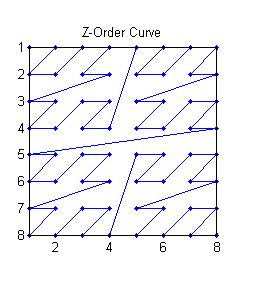
\includegraphics[width=0.5\textwidth]{z-curve.JPG}
\caption{Z-order curves}
\end{figure}
Basically, if one traces the above curve, the 27th point on the curve will end up at the coordinate (3, 5). Treat the z-value as primary key and use B-Tree to index it. Now that we have converted our multidimensional data to 1-d points, the next step is to see how spatial queries can be executed on this data set. To find city at a location, say, (0,3), the z-value which is indexed (5 in this case) is looked up and the city name in the table is retrieved. For range queries, simply computing the ranges of z-values. For nearest neighbor, traverse the B-tree and find nearest neighbor with respect to z-values and do a range query. Using different techniques, other query types can also be performed on the 1-d data we have stored in our database \cite{orenstein1986spatial}.  
\subsection{Spatial data indexing techniques}
\subsubsection{R-Tree}
The first indexing structure that we surveyed was R-Tree. Antonin Guttman and Micheal Stonebreaker\cite{guttman1984r} proposed R-Tree in 1984 which is used to index multidimensional spatial data. The spatial data objects are indexed using a minimum bounding rectangle hierarchically. Each entry in R-Tree is represented as a \{rectangle, pointer\} pair. In leaf nodes, the pointer refers to the spatial data object in secondary storage and rectangle indicates the minimum bounding rectangle encompassing the spatial object. The intermediate nodes contain a reference to the child node (pointer) and the minimum bounding rectangle covering all the spatial objects in the child node (rectangle). R-Tree is balanced, i.e. all the leaf nodes are the same height from the root node. R-Tree satisfies the property that $m \leq M/2$, where \textit{m} denotes the minimum number of entries and \textit{M} denotes the maximum number of entries in a given node. So every intermediate node has between \textit{m} and \textit{M} nodes unless it's a root node\cite{guttman1984r}.\\

\begin{figure}[h!]
\centering
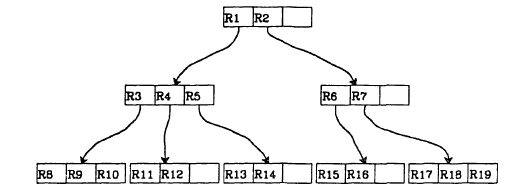
\includegraphics[width=0.5\textwidth]{R-Tree1.png}
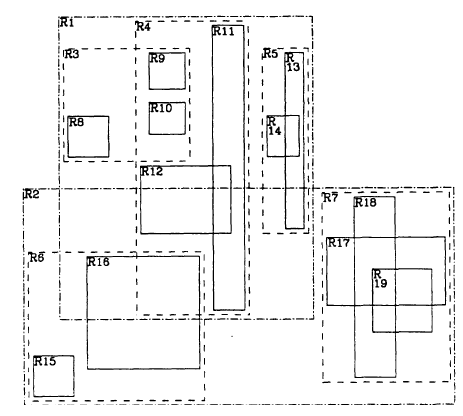
\includegraphics[width=0.5\textwidth]{R-Tree2.png}
\caption{R-Tree \cite{guttman1984r}}
\end{figure}

The update algorithm in R-Tree makes life easier for searches as the tree is balanced after every update operation thereby eliminating irrelevant regions during search. After every addition the algorithm invokes methods to expand the tree and split nodes if necessary in case of addition. The deletion method is followed by a CondenseTree action which adjusts the rectangles so that they cover minimal area and propagates the deletion toward the root. These methods make it easier for search to identify the nodes that wouldn't cover the given window range. R$^\star$-Tree is a variant of R-Tree with increased cost of insertion but better query performance\cite{guttman1984r}.\\

R-Trees are effective when performing queries like spatial join and nearest neighbor. Brinkhoff, kriegel and Seeger \cite{brinkhoff1993efficient} describe a basic algorithm for spatial join using R$^\star$-Tree. Their algorithm leverages the fact that if two directory entries don't have any overlapping rectangles, then the subtrees originating from those entries need not be considered\cite{brinkhoff1993efficient}. Ruossopoulos, Kelley and Vincent \cite{roussopoulos1995nearest} use two metrics in implementing nearest neighbor queries. The optimistic approach uses the minimum distance between the spatial object and given point. The pessimistic approach takes the minimum of maximum possible distance from the point to the MBR containing the spatial object. These approaches denote the lower and upper bound for the actual distance\cite{roussopoulos1995nearest}\\

\subsubsection{GiST}
A good survey of GiST is provided by Hellerstein, Naughton and Pfeffer\cite{hellerstein1995generalized}. GiST stands for Generalized Search Trees is an extension of search tree data structures which supports many queries and new data types can be easily extended from GiST. The nodes in GiST contain entries with \{predicate,pointer\} pairs. The leaf nodes contain pointers to the data in disk and the predicate denotes the search key used. Non-leaf nodes contain pointers which point to subsequent subtrees or child nodes and the predicate consists of search key used. An important property of GiST is that the predicate can have any number of variables as long as single tuple can be referenced from the pointer satisfying the corresponding predicate. The keys in predicates include range of integers in case of B$^+$- Trees or MBR in case of R-Trees.\\

GiST supports union and intersection functions among others which can be used to find a geometric union or check for overlaps between bounding boxes or polygons. The search algorithm employed by GiST uses a simple recursive approach of checking the predicate's validity at every hierarchical level. In case of range or window queries multiple values may give an exact match for the given predicate. GiST also offers FindMin and Next methods which can be leveraged when linearly ordered domains are in use. These methods coupled with search algorithm provide an efficient implementation. The insert and delete operations maintain the balance of the tree by splitting nodes and balancing them while insertion and condenseTree after deletion akin to those in R-Trees\cite{hellerstein1995generalized}.
The aforementioned data structures become imperative when dealing with spatial data, the principal reason for this survey.

\subsubsection{K-D Tree}

K-d trees are space portioning trees for organizing points in k-dimensional space. They are similar to extended binary partitioning trees and are mainly used in multidimensional search queries like range searches and nearest neighbor. K-d trees are traditionally built using a greedy, top-down approach using surface area heuristic to evaluate split candidates. K-d trees are binary trees where every node is a k-dimensional point. A splitting hyper-plane is generated by the internal nodes (non-leaf nodes) which divides the space into half-spaces. The points to the left and right of this half-space are represented by the left and right subtrees respectively. In k dimensions, record is represented by k keys. Any one these can serve as discriminator for partitioning the file representing the k-d tree. 

\begin{figure}[h!]
\centering
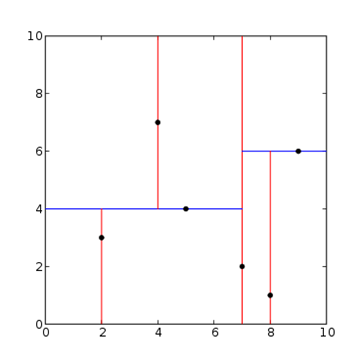
\includegraphics[width=0.5\textwidth]{KDTree.png}
\caption{K-D Tree}
\end{figure}


Points are inserted by selecting a median of points being put in the subtree. This is done using a greedy approach starting from the root node. K-d trees are efficient when used with nearest neighbor queries. The search is done efficiently by using tree properties to reduce unwanted search space. The search starts off at the root node and propagates down toward the leaf nodes. The leaf node thus reached is assigned as the “current best” node. The recursion is now backtracked and if the current node is closer than the current best then it is assigned as the new current best. The search also considers points lying on the other side of the splitting plane that might be closer to current best. This is done by splitting the hyperplane around the search point that has a radius equivalent to the current best distance. As the algorithm reaches the root node, the search is terminated. Friedman at al.\cite{friedman1977algorithm} propose optimizations to the k-d tree by adjusting the discriminating key value and partition at each internal (non-leaf) nodes.
 
Range searches can also be implemented effectively with k-d trees. K-d trees are mainly used with point datasets rather than polygon datasets. This is because k-d tree doesn’t allow any overlap of the node boundaries, which might not support any overlapping polygons in a dataset. Another drawback of k-d tree is that it doesn’t work well with high dimensional data. Unless the number of points is way more than the dimensionality, k-d just uses exhaustive search to give out nearest neighbor results. 


\subsubsection{Quad Tree}

Quadtrees are hierarchical data structures based on recursive decomposition. They are usually differentiated based on the type of data they represent, the decomposition principle applied or the resolution. They are used to represent point, data, regions, curves or contours. The internal nodes of a quadtree have exactly four children which are assigned capacities. Once this capacity is reached, they spill over. In a quadtree, each node represents a bounding box covering some part of the space being indexed, the root node covering the whole area. We are more concerned with region quadtree which divides given area into four quadrants which is recursively divided in the same way. The region quadtree is similar to an extended binary search tree for two dimensions.\cite{samet1984quadtree} 

\begin{figure}[h!]
\centering
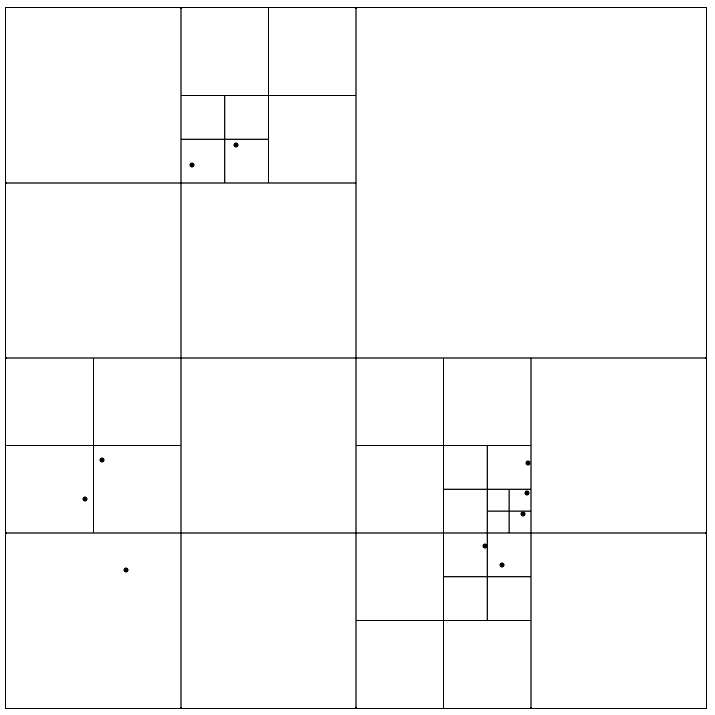
\includegraphics[width=0.5\textwidth]{quadtree2.png}
\caption{Quadtree}
\end{figure}

The insertion into quadtree starts off at the root node determining the quadrant containing the point. The quadrants are recursively traversed to find the leaf node. The point or part of the region is then added to the node’s existing set of points. If there is a spillover (number of entries in the point exceed a minimum threshold) the node is split into four children. The initial leaf node now becomes an internal node. Finding the nearest neighbor is achieved by a top-down recursive algorithm. We explore the subtree that contains the said point at each level of recursion. Once the leaf node is reached, the distance to its nearest neighbor is calculated. As we unwind the recursion we look for any overlap in the higher levels between the subtrees being considered. 

Quadtrees can also be used to represent rectangle data. They serve as an approximation for polygons, curves and regions through a rectilinear minimum bounding object. The approximation gives an indication of the existence of an object. The exact boundaries are also stored, but they are used accessed only if greater precision is needed. Kothuri et al.  \cite{kothuri2002quadtree} provide a good survey of index comparisons on oracle spatial. They compare quadtree and R-Tree on scalability, tiling level with quadtrees, approximations in R-Trees and mainly the index creation.\cite{kothuri2002quadtree} 



\section{Evaluation}
A framework for presentation and comparison of indexing schemes would provide a standard based on which indexes could be evaluated. Some of the important tests when it comes to evaluation are \textit{scalability, query evaluation speed, CPU time, disk traffic, memory requirements and index construction speed}.  All of these factors can be backed up by an experiment which itself should be reproducible and based on standard sets of data and queries. A short description of each of the important factors follows in this sections. This has been done in order to get a quick overview of the objectives involved in each of the test.
\begin{itemize}
\item \textbf{Scalability:} Consider average costs as well as best and worst case costs. Asymptotic analysis will show what happens when the size of data is increased greatly. Scaling will show the relative performance for different data sizes which helps us gauge performance.
\item \textbf{Query evaluation speed:} Index speed is discussed in the context of a class of queries. It is important to describe speed in terms of the performance of available hardware.  It is also important that tests start without any caching or previously stored computation in order for the comparison to remain fair.
\item \textbf{Memory requirements:} There needs to be a mention of how the indexing uses the memory and its memory use on other factors. Sometimes indexes can be completely held in memory and other times require more space that can be obtained only from disk. These specifications need to be considered.
\item \textbf{Index construction:} It is vitally important that for any indexing scheme, the time taken to construct that index should be done in a reasonable time. Temporary space allocations during index construction is also an important consideration. 
\end{itemize}
Our project takes into account the above factors and some not-to-do's mentioned in the paper and performs comparison analysis on a standard data set,to provide a fair environment under which the indexing techniques will be compared \cite{zobel1996guidelines}.

\section{Experiment}
\subsection{System description}
The spatial database system considered for this evaluation experiment was PostgreSQL with POSTGIS. The POSTGIS extension provides spatial functions like geometry data types, area, distance, intersection, union and more.\\
PostgreSQL is an Object-Relational Database system. POSTGIS is spatial database extender for POSTGRESQL object-relational database system. POSGIS allows geographic objects to run location queries in SQL.\\
Extra types such as geometry are added by POSGIS to the PostgreSQL database. These spatial types are added with functions, operators and indexing structures which makes PostgreSQL Database Management System fast, feature-plenty and robust spatial DBMS

\subsection{Data set}
In order to use POSTGIS with POSTGRESQL it is required that the data is in a form that can be worked with these two. In our case, the format chosen was tables in the form of \textit{shapefiles}. According to the makers of ArcGIS \textit{a shapefile is an Esri vector data storage format for storing the location, shape, and attributes of geographic features. It is stored as a set of related files and contains one feature class}.\\

The spatial data set used in this experiment is the benchmark data from the New York City Government open database. It includes point data: subway stations, line data: streets and subway lines, polygon data: boroughs and neighborhoods and some non-spatial data like demographic data. The data set contains four tables:\\
\subsubsection{NYC_CENSUS_BLOCKS}
This contained 38794 non-spatial population records.
\begin{table}[!ht]
\begin{tabular}{ |l|l| }
\hline
Parameter & description\\
\hline
blkid & Unique identity for every census block\\
\hline
popn_total & Total population in the census block\\
\hline
popn_white & Total white population\\
\hline
popn_black & Total black population\\
\hline
popn_asian & Total asian population\\
\hline
popn_native & Total native population\\
\hline
popn_other & Total other population\\
\hline
boro_name & Name of the borough in New York\\
\hline
geom & Polygon Boundary of the borough\\
\hline
\end{tabular}
\caption{NYC CENSUS BLOCKS}
\label{tab:census blocks}
\end{table}

\subsubsection{NYC_NEIGHBORHOODS}
This table contained 129 polygon records
\begin{table}[!ht]
\begin{tabular}{ |l|l| }
\hline
parameter & description\\
\hline
name & Name of the neighborhoods\\
\hline
boroname & Name of the boroughs in New York \\
\hline
geom & Polygon boundary of the neighborhood\\
\hline
\end{tabular}
\caption{NYC NEIGHBORHOODS}
\label{tab: neighborhoods}
\end{table}
\subsubsection{NYC_STREETS}
This contained 10991 line records
\begin{table}[!ht]
\begin{tabular}{ |l|l| }
\hline
parameter & description\\
\hline
name & Street names\\
\hline
oneway & Is the street one way? Yes/No \\
\hline
type & The type of the tree-- \\ \ & primary/secondary/motorway\\
\hline
geom & Geometry of the line street\\
\hline
\end{tabular}
\caption{NYC STREETS}
\label{tab: streets}
\end{table}
\subsubsection{NYC_SUBWAY_STATIONS}
\begin{table}[!ht]
\begin{tabular}{ |l|l| }
\hline
parameter & description\\
\hline
name & Station name\\
\hline
borough & Name of the borough in New York \\
\hline
routes & Subway lines that run through this station\\
\hline
transfers & lines you can transfer to, via this station\\
\hline
express & Stations where express trains stop -- Yes/No\\
\hline
geom & Geometry of the line street\\
\hline
\end{tabular}
\caption{NYC STREETS}
\label{tab: streets}
\end{table}

\subsection{Types of queries}
For the purpose of this project we identified some important query types, performance on which were used as the parameters to compare the indexing techniques. These queries were picked based on the fact that there was enough overlap between these query types and the types of operations that a spatial indexing technique is expected to solve according to our survey.
\subsubsection{k-NN queries}
The \textit{nearest neighbor} queries handled in this project fall under the category of \textit{boolean k-NN} queries. These queries can be described as those asking for a set of values, ordered based on some parameter, which satisfy the criteria that it contains the keyword(s) specified in the query. For instance, in our New York City data set, a sample k-NN query would be to return all the subway stations ordered by closest to farthest from a particular street or neighborhood.
\subsubsection{Geometry queries}
We 
\subsection{Queries}
\subsubsection{Index Creation}
The dataset considered for this project was indexed using the following techniques:
\begin{itemize}
\item \textbf{GiST (R-Tree)}: CREATE INDEX \textit{nyc_subway stations_geom_gist} ON \textit{public.nyc_subway_stations} USING \textit{gist(geom)}
\item \textbf{B-Tree GiST}: CREATE INDEX \textit{nyc_subway stations_geom_gist} ON \textit{public.nyc_subway_stations} USING \textit{b_tree(st_x(geom))}
\item \textbf{K-D TRee}: CREATE INDEX \textit{nyc_subway stations_geom_gist} ON \textit{public.nyc_subway_stations} USING \textit{sp_gist(POINT(st_x(geom),st_y(geom))) kd_point_ops} 
\item \textbf{Quad TRee}: CREATE INDEX \textit{nyc_subway stations_geom_gist} ON \textit{public.nyc_subway_stations} USING \textit{sp_gist(POINT(st_x(geom),st_y(geom))) quad_point_ops} 
\end{itemize}
\subsubsection{Geometry Functions}
Geometry queries that were evaluated in this experiment were of the following type:\\\\
SELECT \textit{name, st_AsText(geom)}\\ 
FROM \textit{nyc_subway_stations} \\
WHERE \textit{name=`Broad Street'} \\\\
SELECT \textit{name, boroname} \\
FROM \textit{nyc_neighborhoods}\\
WHERE \textit{ST_Intersects(geom, ST_GeomFromText('POINT(583571 4506714)',26918))}
\subsubsection{Boolean Range Query}
The boolean range queries that were evaluated in this experiment were of the following type:
SELECT \textit{nyc_subway_stations.name, nyc_neighborhoods.name} \\
FROM \textit{nyc_subway_stations,nyc_neighborhoods} \\
WHERE \textit{(nyc_neighborhoods.name = 'East Village' or nyc_neighborhoods.name = 'West Village')} \\
AND \textit{nyc_neighborhoods.geom \& \& nyc_subway_stations.geom}
\subsubsection{Joins}
The queries to perform and evaluate joins in this experiment were of the following type:\\\\
SELECT \textit{nyc_subway_stations.name,nyc_neighborhoods.name, nyc_neighborhoods.boroname}\\
FROM \textit{nyc_neighborhoods}\\
JOIN \textit{nyc_subway_stations}\\
ON \textit{ST_Contains(nyc_neighborhoods.geom, nyc_subway_stations.geom)}
\subsubsection{K-NN queries}
SELECT s.name, s.routes\\
FROM nyc_subway_stations\\
AS s JOIN nyc_neighborhoods\\
AS n ON ST_Contains(n.geom, s.geom)\\
WHERE n.name = 'Bensonhurst' \\\\
%
The above query identifies \textit{which subway station is nearest to the ‘Bensonhurst' neighborhood.}
An example of another type of k-NN query where we don't have prior knowledge about the results we may get:\\
SELECT \textit{streets.gid, streets.name}\\
FROM \textit{nyc_streets streets, nyc_subway_stations subways}\\
WHERE \textit{subways.name = 'Cortlandt St'}\\
ORDER BY \textit{ST_Distance(streets.geom, subways.geom)}\\
ASC LIMIT 1;



\section{Results and analysis}
In this section we report on the different indices covered in the previous sections. First, we present the space occupied by each index when indexing the geometry column available in our data set. Then, we present the time taken to construct each index. The space-occupied and the index build time are important factors when it comes to huge data sets which is the norm for spatial data sets. Space constraints and memory constraints are important factors in spatial data processing and hence it is crucial to include these aspects into consideration when selecting indexes for an application that involves spatial data processing. Then, we present the results of query processing performance of the GiST, B-Tree, kd Tree and Quadtree indexing on our data sets. Specifically, we run different spatial queries like the nearest neighbor query, range and containment queries, spatial joins and simple spatial relationship based queries.
\subsection{Space and Time requirements}
\begin{table}
\begin{tabular}{ |l|l| }
\hline
Index & Size on disk (in KB)\\
\hline
GiST & 72\\
\hline
B-Tree & 64\\
\hline
K-D Tree & 96\\
Quad Tree & 96\\
\hline
\end{tabular}
\caption{Table listing indices and their sizes on disk}
\label{tab:index}
\end{table}
Table \ref{tab:index} presents space requirements for each index. As we can see, the space occupied by the B-Tree index is lowest because we just have to index either the x-coordinate of the points in our data set or the y-coordinate of the points based on whichever coordinate we prefer to index. Comparing the space usage of R-Tree vs space partitioning techniques like the kd-tree and the Quadtree we can see the R Tree has comparatively lower usage of space. This is because for storage of points in the kd-Tree and Quadtree generates many tiles for the point geometry in order to separate points into their own nodes.

Index Creation times as can be seen in the figure ___ shows that B-Tree takes a long time to index the data. K-d tree has the shortest index creation time among all the techniques. The reason for this is that indexing point data types is most suited for k-d tree which basically partitions the plane recursively based on a median and builds the tree. R-Tree index takes a little longer because it is a balanced tree and the time-taken to balance the tree is added to the index creation time. 
\subsection{Query Execution Time}
As can be observed from the figure ___, R-Tree based GiST index takes the least amount of time when averaged for geometry functions like ST_Dwithin and ST_intersects. This is easy to comprehend because points and polygons are stored as Minimum bounding rectangles and polygons and points that intersect and are closer together are also the same way in the R-Tree. In B-Tree the points are sorted based on one coordinate and the execution time is comparable as sorting leads to better search results when it comes to geometric function based queries.  However, B-Tree is the slowest of all techniques when implementing geometry functions even though the time is comparable to other techniques.\\\\

For Spatial Joins, the performances of all the indices are comparable. This is mainly because when we join the table consisting of point-based datasets and polygon based datasets we employ the GiST indexing on the polygon dataset and vary the indexing on the point data (subway_stations). The impact of indexing the polygon seemed to have had a greater impact than the indexing on the point data. This shows the versatility and ease of an R-Tree based GiST index compared to the other techniques. Since only the GiST was capable of indexing polygons, the rest of the techniques were not used to evaluate the performance. However, without using an index on the polygon, we found that the k-d tree based technique was faster when it came to spatial joins. Again this is due to the suitability of k-d tree to split the plane and index points in 2 dimensions. However, the GiST index also has comparable performance and the ease of its use could potentially make it preferable for applications that involve high number of spatial joins especially if the number of dimensions are higher. \\

For nearest neighbor queries all the indexes had comparable performance. Within this performance scenario, the R-Tree based GiST performed the best. This is intuitive as the R-Tree stores the point space and maps it as is in its index. For the space partitioning trees like K-D tree and QuadTree the points are split and nearest neighbor in the actual multidimensional space may not map to nearby nodes in the index tree representation. One expects these techniques to be significantly slower than the multidimensional R-Tree index but because the search with an average complexity of O(log n) where n is the number of nodes in the tree with each node containing its own point the indexing compares to the R-Tree index. Similar to the join, k-d trees and quadtrees are not suited for higher dimension nearest neighbor because of the inherent complexity of constructing the trees with increase in dimensions.  

\section{Conclusion}
We surveyed and evaluated the performance of four different spatial indexing techniques that may help users understand the different characteristics of each of the indexes and their strong suits. When choosing the type of index to use on datasets within application, the reader can use the results to select the appropriate index based on the type of spatial query that is most likely to be performed when using the application. The paper evaluated the basic spatial queries like joins, nearest neighbor searches, range queries that are fundamental types of spatial queries in use today for different applications. We found that the consistent performance and ease of use of R-Tree based GiST index has the highest utility. The k-d tree based index almost always outperforms its space-partitioning counterpart Quadtree index and could be preferred when the data is of two-dimensions and dealing mainly with point-based data.   It has strong performance in the spatial range, containment and intersection queries and could be used as the main index in the scenario where the application mainly uses range queries such as for finding subway stations within a neighborhood or all restaurants in a neighborhood etc. Varying the selectivity factor in the range query, we found that the k-d tree performs the best as selectivity decreases. We would say that the R-Tree based GiST is natural and easy to implement in a Postgres database and its consistent performance makes it the best contender. It’s capability to index points as well as lines and polygons makes it versatile. For space partitioning trees like k-d tree and QuadTree data has to be modified to fit the tree whereas for the GiST there is no need for any processing of data which makes it easier for application developers. 

%\end{document}  % This is where a 'short' article might terminate

%ACKNOWLEDGMENTS are optional
%
% The following two commands are all you need in the
% initial runs of your .tex file to
% produce the bibliography for the citations in your paper.
\bibliographystyle{abbrv}
\bibliography{sigproc}  % sigproc.bib is the name of the Bibliography in this case
% You must have a proper ".bib" file
%  and remember to run:
% latex bibtex latex latex
% to resolve all references
%
% ACM needs 'a single self-contained file'!
%
%APPENDICES are optional
%\balancecolumns
% This next section command marks the start of
% Appendix B, and does not continue the present hierarchy
%\balancecolumns % GM June 2007
% That's all folks!
\end{document}
